\chapter{\IfLanguageName{dutch}{Boomi}{Boomi}}
\label{ch:Boomi}

De eerste integratie tool waarvan de resultaten zullen besproken worden is Boomi. Hieronder worden de requirements individueel besproken en krijgen ze een score tussen 1 (voldoet niet aan de verwachtingen) en 5 (voldoet aan alle verwachtingen) toegewezen. Op het einde van het hoofdstuk worden alle requirements en hun scores samengevat en weergegeven in een tabel met enkele extra berekeningen om het vergelijkingsproces te vereenvoudigen.

\section{Requirements}%
\label{RequirementsBoomi}

\subsection{Must have}%
\label{MustHaveBoomi}

\textbf{Veiligheid en betrouwbaarheid: De tool moet voldoen aan de relevante beveiligingsnormen (Welbekende ISO-normen, data-encryptie, Europese GDPR-wetgeving compliance).}

\vspace{\baselineskip}

Boomi staat algemeen bekend als een veilige en betrouwbare tool voor enterprise data integratie. Het beschikt over verschillende certificeringen zoals ISO 27001 voor informatiebeveiliging beheer, SOC 1 en SOC 2 Type 2 voor onafhankelijke controles van interne processen en gegevensbescherming en voldoet tenslotte aan de eisen van de Europese GDPR-wetgeving. Boomi maakt ook gebruik van encryptie bij het transporteren van data aan de hand van TLS en SSL. Op vlak van authenticatie en autorisatie maakt Boomi gebruik van Single Sign-on (SSO) via SAML 2.0 en maakt het ook gebruik van Role-based access control (RBAC) voor een onoverzichtelijke en veilige toegangscontrole.

Voor dit requirement scoort Boomi een 4.

\vspace{\baselineskip}

\textbf{Uitbreidbaarheid: De tool moet eenvoudig uitbreidbaar zijn met nieuwe modules en integraties naarmate de organisatie groeit.}

\vspace{\baselineskip}

Boomi kan hun systemen perfect uitbreiden of inperken naargelang de wensen van het bedrijf. De schaal van de uitbreidbaarheid of de inperking zal afhankelijk zijn van de voorwaarden in het contract dat Boomi vooraf heeft afgesproken met het bedrijf. Bij grote wijzigingen kan het zijn dat het contract herzien moet worden en daardoor ook opnieuw onderhandeld moet worden met Boomi.

Voor dit requirement scoort Boomi een 4.


\vspace{\baselineskip}

\textbf{Integratie van meerdere systemen: Het platform moet in staat zijn om verschillende applicaties en systemen met elkaar te verbinden (zoals ERP, CRM, HRM, legacy-systemen, databases) met elkaar te verbinden.}

\vspace{\baselineskip}

Boomi is in staat om verschillende applicaties en systemen met elkaar te kunnen verbinden. Sommige systemen zullen vlot en makkelijk met elkaar in verbinding gebracht kunnen worden, voor andere zullen custom componenten aangemaakt moeten worden om het verkeer van deze data transacties vlot te doen verlopen. Door het grote aanbod aan flexibele en aanpasbare componenten zou het mogelijk moeten zijn om bijna iedere soort data-integratie te kunnen creëren.

Voor dit requirement scoort Boomi een 4.

\vspace{\baselineskip}

Hieronder de aangemaakte data integraties van de proof of concept:

\begin{figure}[H]
    \centering
    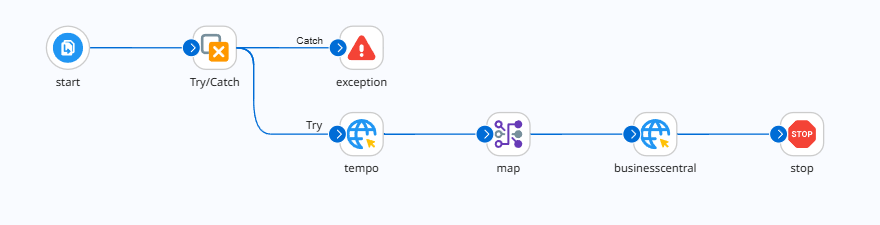
\includegraphics[width=\textwidth,height=\textheight,keepaspectratio]{../bachproef/images/Boomi_AtlassianTime.png}
    \caption{Boomi: data integratie tussen Atlassian Tempo en Microsoft Business Central}
\end{figure}

\begin{figure}[H]
    \centering
    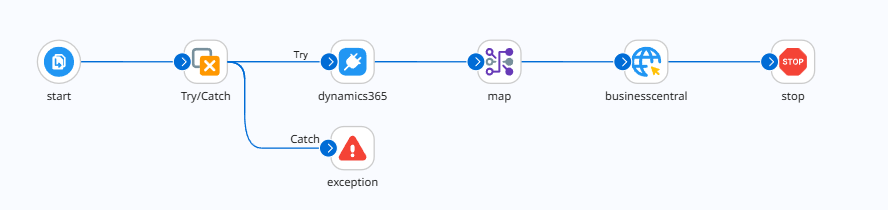
\includegraphics[width=\textwidth,height=\textheight,keepaspectratio]{../bachproef/images/Boomi_Quote_Creation.png}
    \caption{Boomi: data integratie tussen Microsoft Dynamics Sales en Microsoft Business Central}
\end{figure}

\begin{figure}[H]
    \centering
    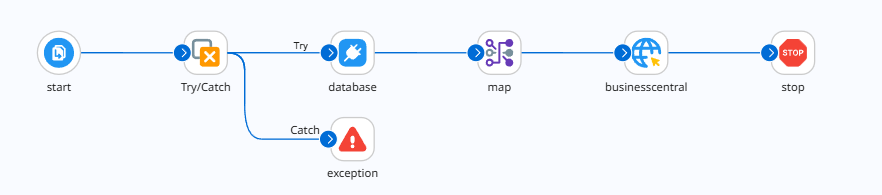
\includegraphics[width=\textwidth,height=\textheight,keepaspectratio]{../bachproef/images/Boomi_Database_BusinessCentral.png}
    \caption{Boomi: data integratie tussen Microsoft SQL Server en Microsoft Business Central}
\end{figure}

\vspace{\baselineskip}

\textbf{Automatisering van processen: Manuele administratieve taken moeten geautomatiseerd kunnen worden om fouten te verminderen en bepaalde processen te versnellen.}

\vspace{\baselineskip}

Boomi beschikt over de mogelijkheid om taken manueel en automatisch uit te voeren. Manuele processen kunnen via de website handmatig uitgevoerd worden. Geplande of tijdgestuurde uitvoeringen kunnen dagelijks, wekelijks, maandelijks of op specifiek geplande dagen automatisch uitgevoerd worden. Tenslotte is het ook mogelijk om processen reactief uit te voeren als een soort event-driven proces aan de hand van webhooks, database triggers of andere events.

Voor dit requirement scoort Boomi een 4.


\vspace{\baselineskip}
\textbf{Data-transformatie: Het platform moet data makkelijk kunnen converteren tussen verschillende formaten en structuren (bijv. XML ↔ JSON, CSV ↔ database records).}

\vspace{\baselineskip}

Boomi beschikt over een mapping component dat het mogelijk maakt om data van verschillende datatypen te converteren naar het gewenste data type. In de mapping component kan er gekozen worden uit de volgende datatypen om te converteren:

\begin{itemize}
    \item XML
    \item JSON
    \item Flat file
    \item EDI
    \item Database (legacy)
\end{itemize}

Voor dit requirement scoort Boomi een 5.


\vspace{\baselineskip}


\textbf{Monitoring en logging: Het systeem moet real-time monitoring en logboek functionaliteiten bieden om fouten en prestaties bij te houden.}

\vspace{\baselineskip}

Boomi biedt de mogelijkheid aan om data integraties te monitoren, controleren en te testen. Met ook de mogelijkheid om errors op te vangen aan de hand van een try/catch systeem of andere vormen van logische poorten indien er iets fout gaat gedurende het proces. Desondanks voelde deze monitoring- en debugging tool beperkter en minder diepgaand aan dan bij de andere data integratie tools.

Voor dit requirement scoort Boomi een 3.


\vspace{\baselineskip}

\subsection{Should have}%
\label{ShouldHaveBoomi}

\textbf{Kostenbeheersing: De tool moet betaalbaar zijn met een transparant kostenmodel (licenties, onderhoud, implementatie).}

\vspace{\baselineskip}

Van alle drie de integratie tools is Boomi het minst transparant over de exacte kosten van hun software en services. Boomi heeft namelijk 2 kostenmodellen waaruit de klant kan kiezen namelijk:

\vspace{\baselineskip}

Een abonnementsstructuur waarbij de klant kan kiezen uit 4 opties naargelang de wensen en de grootte van het bedrijf hierbij wordt er geen exacte prijs op voorhand aangegeven en moet er onderhandeld worden met het sales team van Boomi voor een abonnement op maakt uit te werken. Hieronder worden de 4 abonnement modellen kort toegelicht voor een idee te geven van hun schaal:

\begin{itemize}
    \item Base Edition: geschikt voor eenvoudige integraties.
    \item Professional Edition: voor meerdere applicaties en basis-API-ondersteuning.
    \item Enterprise Edition:  gericht op complexe integraties, API management, en EDI.
    \item Enterprise Plus / Ultimate:  voor organisaties met zeer hoge schaal- en governance-eisen.
\end{itemize}

Als tweede betaaloptie biedt Boomi ook nog een pay-as-you-go model aan waarbij de klant maandelijks 99 dollar moet betalen als basisprijs + extra verbruikskosten afhankelijk van het verbruik dat het bedrijf maandelijks maakt. De exacte bedragen voor deze verbruikskosten worden helaas niet op de website weergegeven en ook hiervoor zal er contact opgenomen moeten worden met het sales team van Boomi.

Tenslotte is er ook de mogelijkheid om Boomi gratis voor 30 dagen uit te proberen om een inkijk te geven in het ecosysteem van Boomi. Na 30 dagen wordt het trial-account wel verwijderd dus hiervoor moet opgelet worden indien er na een testfase zou gekozen worden om Boomi verder te gebruiken.

Voor dit requirement scoort Boomi een 2.

\vspace{\baselineskip}

\textbf{Schaalbaarheid: De tool moet eenvoudig schaalbaar zijn naargelang de wensen van de organisatie.}

\vspace{\baselineskip}

Boomi kan hun systemen perfect schalen naargelang de wensen van de klant. Deze schaalbaarheid is wel afhankelijk van het vooraf afgesproken contract dat het bedrijf heeft met Boomi. Het is perfect mogelijk om de schaalbaarheid te wijzigen indien nodig, maar hiervoor kan het zijn dat bedrijven contact moeten opnemen met Boomi om hun contract te wijzigen naargelang de grootte van de schaal die gewijzigd moet worden.

Voor dit requirement scoort Boomi een 4.


\vspace{\baselineskip}

\textbf{Connectoren en adapters: Het platform moet kant-en-klare connectoren bieden voor veelgebruikte systemen (bijv. SAP, Microsoft Dynamics, Oracle).}
\vspace{\baselineskip}

Boomi beschikt over een enorm aanbod aan kant-en-klare connectoren om connecties te maken met welgekende systemen zoals SAP, Amazon, Microsoft Dynamics, Oracle, Salesforce, Azure en andere grote bedrijven. Toch beschikt Boomi niet over alle connectoren die Axians zou nodig hebben. Zo is er voor Atlassian in geen enkele vorm een beschikbare kant-en-klare connector beschikbaar en moest deze zelf aangemaakt worden. Voor andere niche systemen zal men waarschijnlijk ook gezien moeten worden om eigen custom connectoren aan te maken.  

Voor dit requirement scoort Boomi een 4.


\vspace{\baselineskip}

\textbf{Prestaties: De tool moet performant zijn bij het uitvoeren van bepaalde veelgebruikte data integraties, maar niet alle data integratie processen.}

\vspace{\baselineskip}

Boomi presteert goed bij standaard en veelvoorkomende data integraties, vooral in cloudomgevingen. Bij minder traditionele, complexere of data intensieve processen kan de performance licht tegenvallen door beperkingen in optimalisatie. Gezien de requirement stelt dat niet alle processen performant moeten zijn, scoort Boomi relatief goed, zolang de focus op de standaardintegraties ligt zoals de data integratie tussen Microsoft Dynamics Sales en Microsoft Business Central.

Voor dit requirement scoort Boomi een 4.

\vspace{\baselineskip}

\textbf{Onderhoudsvriendelijkheid: De tool moet eenvoudig te updaten en te onderhouden zijn met minimale downtime.}

\vspace{\baselineskip}

Boomi biedt een service level agreement van 99.99\% uptime aan en houdt ook een revisie geschiedenis aan dat aantoont welke aanpassingen er zijn gemaakt door wie en ook wanneer deze wijzigingen plaatsvonden. Eerdere versies van een data integratie kunnen aangevraagd worden en ook opnieuw bewerkt worden.

Voor dit requirement scoort Boomi een 4.

\vspace{\baselineskip}

\subsection{Could have}%
\label{CouldHaveBoomi}

\textbf{Hybrid en multi-cloud ondersteuning: Het platform moet applicaties kunnen integreren die draaien in verschillende omgevingen (on-premise, private cloud, public cloud).}

\vspace{\baselineskip}

Boomi biedt een uitgebreide ondersteuning voor hybrid en multi-cloud integraties, met sterke tools voor connectiviteit, deployment en beheer. Het platform is gebruiksvriendelijk, maar kan in zeer complexe of sterk gereguleerde omgevingen nog enige aanpassing of extra tooling vereisen.

Voor dit requirement scoort Boomi een 4.

\vspace{\baselineskip}

\textbf{Low-code / no-code interface: Het platform beschikt over een low-code of no-code interface voor het aanmaken van data integraties.}

\vspace{\baselineskip}

Boomi biedt sterke low-code capaciteiten en een gebruiksvriendelijk interface die veel integraties mogelijk maakt zonder diepgaande technische kennis. Langs de no-code kant lijkt het requirement niet volledig haalbaar bij complexere scenario's en voor meer geadvanceerde data integraties is technische expertise tamelijk nodig.

Voor dit requirement scoort Boomi een 4.

\newpage

\begin{landscape}

\subsection{Eindoverzicht}%
\label{EindoverzichtBoomi}

\begin{table}[H]
\centering
\resizebox{\linewidth}{!}{% resize the table to fit page width
\begin{tabular}{|ll|}
\hline
\multicolumn{1}{|l|}{\textbf{Requirements uit de requirementsanalyse}}                                                                                                                                                     & \textbf{Score tussen 1 en 5} \\ \hline
\textbf{Must have}                                                                                                                                                                                                         &                              \\ \hline
\multicolumn{1}{|l|}{Veiligheid en betrouwbaarheid: De tool moet voldoen aan de relevante beveiligingsnormen (Welbekende ISO-normen, data-encryptie, Europese GDPR-wetgeving compliance).}                                 & 0                            \\ \hline
\multicolumn{1}{|l|}{Uitbreidbaarheid: De tool moet eenvoudig uitbreidbaar zijn met nieuwe modules en integraties naarmate de organisatie groeit.}                                                                         & 0                            \\ \hline
\multicolumn{1}{|l|}{Integratie van meerdere systemen: Het platform moet in staat zijn om verschillende applicaties en systemen met elkaar te verbinden (zoals ERP, CRM, HRM, legacy-systemen, databases) met elkaar te verbinden.} & 0                            \\ \hline
\multicolumn{1}{|l|}{Automatisering van processen: Manuele administratieve taken moeten geautomatiseerd kunnen worden om fouten te verminderen en bepaalde processen te versnellen.}                                       & 0                            \\ \hline
\multicolumn{1}{|l|}{Data-transformatie: Het platform moet data makkelijk kunnen converteren tussen verschillende formaten en structuren (bijv. XML ↔ JSON, CSV ↔ database records).}                                      & 0                            \\ \hline
\multicolumn{1}{|l|}{Monitoring en logging: Het systeem moet real-time monitoring en logboek functionaliteiten bieden om fouten en prestaties bij te houden.}                                                              & 0                            \\ \hline
\textbf{Should have}                                                                                                                                                                                                       &                              \\ \hline
\multicolumn{1}{|l|}{Kostenbeheersing: De tool moet betaalbaar zijn met een transparant kostenmodel (licenties, onderhoud, implementatie).}                                                                                & 0                            \\ \hline
\multicolumn{1}{|l|}{Schaalbaarheid: De tool moet eenvoudig schaalbaar zijn naargelang de wensen van de organisatie.}                                                                                                      & 0                            \\ \hline
\multicolumn{1}{|l|}{Connectoren en adapters: Het platform moet kant-en-klare connectoren bieden voor veelgebruikte systemen (bijv. SAP, Microsoft Dynamics, Oracle).}                                                     & 0                            \\ \hline
\multicolumn{1}{|l|}{Prestaties: De tool moet performant zijn bij het uitvoeren van bepaalde veelgebruikte data integraties, maar niet alle data integratie processen.}                                                    & 0                            \\ \hline
\multicolumn{1}{|l|}{Onderhoudsvriendelijkheid: De tool moet eenvoudig te updaten en te onderhouden zijn met minimale downtime.}                                                                                           & 0                            \\ \hline
\textbf{Could have}                                                                                                                                                                                                        &                              \\ \hline
\multicolumn{1}{|l|}{Hybrid en multi-cloud ondersteuning: Het platform moet applicaties kunnen integreren die draaien in verschillende omgevingen (on-premise, private cloud, public cloud).}                              & 0                            \\ \hline
\multicolumn{1}{|l|}{Low-code / no-code interface: Het platform beschikt over een low-code of no-code interface voor het aanmaken van data integraties.}                                                                   & 0                            \\ \hline
\multicolumn{1}{|l|}{\textbf{Gemiddelde}}                                                                                                                                                                                  & 0                            \\ \hline
\multicolumn{1}{|l|}{\textbf{Mediaan}}                                                                                                                                                                                     & 0                            \\ \hline
\end{tabular}
}
\caption{Boomi: Beoordeling van requirements op een schaal van 1 tot 5}
\end{table}

\end{landscape}